\documentclass[11pt]{article}
\usepackage{test02-style}
\homeworknumber{2}
\studentname{J.C. Vaught}
\studentstatus{Graduate}
\duedate{Oct. 28, 2026}
\lstdefinestyle{hwmatlab}{language=Matlab,
  backgroundcolor=\color{lightgray},
  basicstyle=\footnotesize\ttfamily\color{black},
  keywordstyle=\color{emchteal}\bfseries,commentstyle=\itshape,
  stringstyle=\color{codeorange},numbers=left,
  numberstyle=\scriptsize\ttfamily,numbersep=8pt,
  columns=fullflexible,keepspaces=true,showstringspaces=false,
  breaklines=true,breakatwhitespace=true,frame=single,
  xleftmargin=1.8em,framexleftmargin=0.4em}
\begin{document}
\makehomeworktitle
\begingroup\small\sloppy\tableofcontents\endgroup
\newpage
\subsection*{Assignment}
\bulletitem{G signifies students that take this class for Graduate Credit; they must do all the items}
\bulletitem{UG students are not required to do the G work, but they may do it for bonus points}
\bulletitem{Problems solved beyond the minimum requirements will be given bonus points.}
\bulletitem{Challenge problems are optional; they will earn bonus points.}
\subsection*{Notes}
\bulletitem{Show your work to obtain partial credit if appropriate}
\bulletitem{Always display input data!}
\bulletitem{Partial credit might be given based on work done and MATLAB codes if they are attached; without them, no partial credit can be given.}
\bulletitem{Display numerical results to three significant digits (four if the first digit is 1).}
\bulletitem{Use SI system of measurement \href{https://en.wikipedia.org/wiki/International_System_of_Units}{reference}}
\bulletitem{Scale units using appropriate prefixes (e.g., nano, micro, milli, kilo, mega, giga, and so on) \href{https://en.wikipedia.org/wiki/Metric_prefix}{reference}}
\bulletitem{Problems solved beyond the minimum requirements will be given bonus points.}
\bulletitem{Challenge problems are optional. They may be solved for extra credit}
\bulletitem{Normalized plots are plots with the \ensuremath{y\text{-axis}} scaled between \ensuremath{-1} and \ensuremath{+1}. A plotted variable is normalized by dividing it by its maximum absolute value}
\subsubsection*{Notations and Abbreviations}
\bulletitem{BVP = boundary value problem}
\bulletitem{EOM = equation of motion}
\bulletitem{FBD = free body diagram}
\bulletitem{FRF = frequency response function}
\bulletitem{IVP = initial value problem}
\bulletitem{LHS = left hand side}
\bulletitem{NLM = Newton’s law of motion}
\bulletitem{ODE = ordinary differential equation}
\bulletitem{PDE = partial differential equation}
\bulletitem{RHS = right hand side}
\subsection*{Test scope}
The supplied test contains questions in A.3--A.5, B.4--B.6, and C.3. The remaining sections state ``Nothing here.''\par
\clearpage
\section{Waves}
\subsection{A.3 Calculate Car Motion on a Wavy Road}
Consider a car traveling on a wavy road. The road surface undulates with an amplitude \ensuremath{a=6\,\mathrm{in}} and a wavelength \ensuremath{\lambda=140\,\mathrm{ft}} that follows a cosine shape. The car is modeled as a spring-mass-damper (Figure~\ref{fig:test02-car}) with natural frequency \ensuremath{f_{n}=0.96\,\mathrm{Hz}} and damping ratio \ensuremath{\zeta=14\%}. The maximum car speed is \ensuremath{v_{\mathrm{max}}=113\,\mathrm{mph}}.\par
\begin{figure}[H]
\centering
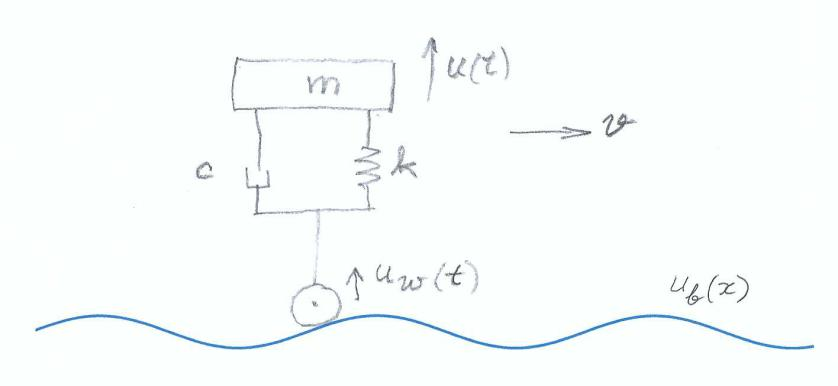
\includegraphics[width=301.85pt]{figures/original/test2-000.jpg}
\caption{Car riding on a wavy road.}
\label{fig:test02-car}
\end{figure}

\taskprompt
\questionitem{1}{Display input data}
\questionitem{2}{Calculate wavy road wavenumber \ensuremath{\gamma}}
\questionitem{3}{Plot the wavy road profile \ensuremath{u_{b}(x)} for \ensuremath{N_{\lambda}=2} wavelengths}
\questionitem{4}{Calculate wavy-road frequency \ensuremath{f_{\mathrm{max}}} for a maximum car speed of \ensuremath{v_{\mathrm{max}}} and define the frequency range \ensuremath{f=\operatorname{linspace}(0,f_{\mathrm{max}},N_{f})} with \ensuremath{N_{f}=2000}}
\questionitem{5}{Plot \ensuremath{\lvert \operatorname{FRF}(f;f_{n})\rvert}. Use datatips to locate the peak response and the matched-frequency response}
\questionitem{6}{Calculate the matched-frequency response value \ensuremath{\lvert \operatorname{FRF}_{n}\rvert}. Compare with the matched-frequency readings at item (5)}
\questionitem{7}{Calculate the car speed \ensuremath{v_{n}} needed to make wavy-road frequency \ensuremath{f} match the car natural frequency \ensuremath{f_{n}}}
\questionitem{8}{Use the conversion \ensuremath{f=v/\lambda} to plot \ensuremath{\lvert \operatorname{FRF}(v ; f_{n})\rvert}. Use datatips on the plot to find:}
\subquestionitem{a}{Find \ensuremath{v_{n}} and \ensuremath{\lvert \operatorname{FRF}_{n}\rvert}, and compare them with the results of items (6) and (7)}
\subquestionitem{b}{Find \ensuremath{v_{\mathrm{cr}}} and \ensuremath{\lvert \operatorname{FRF}_{\mathrm{max}}\rvert}}
\subquestionitem{c}{The limit speed \ensuremath{v_{\mathrm{limit}}} for which the motion amplification is limited to \ensuremath{\lvert \operatorname{FRF}_{\mathrm{lim}}\rvert =1.5}}
\questionitem{9}{Graduate work. Find the road wavelength \ensuremath{\lambda_{\mathrm{new}}} that will make \ensuremath{v_{\mathrm{cr}}=30\,\mathrm{mph}}}
\questionitem{10}{Graduate work. Repeat items (5) through (8) for a car with worn-out shocks that provide only \ensuremath{\zeta=10\%}, and compare the two cases}
\clearpage
\subsection*{Solution to A.3}
\textbf{A.3.1. Input data.} I measure the body coordinate $u(t)$ and road coordinate $u_b(t)$ upward from static equilibrium. The spring and damper act through their relative deformation, so the wheel displacement is the excitation input. The supplied diagram therefore represents base displacement excitation rather than an applied force.

{\begin{center}\small\begin{tabular}{@{}lrl@{}}
\toprule\noalign{}
Quantity & Value & Unit \\
\midrule\noalign{}
$a$ & 0.1524 & m \\
$\lambda$ & 42.672 & m \\
$f_n$ & 0.960 & Hz \\
$\zeta$ & 0.140 & 1 \\
$v_{\max}$ & 50.5155 & m/s \\
$N_\lambda$ & 2 & wavelengths \\
$N_f$ & 2000 & points \\
$|H|_{\mathrm{lim}}$ & 1.50 & 1 \\
\bottomrule\end{tabular}\end{center}}

For the equations of motion, the spring and damper forces depend on $u-u_b$ and $\dot u-\dot u_b$. Newton's law consequently gives
\[
m\ddot u+c(\dot u-\dot u_b)+k(u-u_b)=0,
\qquad
m\ddot u+c\dot u+ku=c\dot u_b+ku_b.
\]
With $\omega_n=\sqrt{k/m}$ and $c/m=2\zeta\omega_n$, harmonic inputs $u_b=\Re\{\hat U_b e^{i\omega t}\}$ give the absolute body-to-road displacement ratio
\[
H(r)=\frac{\hat U}{\hat U_b}
=\frac{1+i2\zeta r}{1-r^2+i2\zeta r},
\qquad r=\frac{f}{f_n}.
\]
Its magnitude is
\[
|H(r)|=\sqrt{\frac{1+(2\zeta r)^2}{(1-r^2)^2+(2\zeta r)^2}}.
\]
The numerator follows from the base-motion terms on the right side of the equation of motion. It is also the absolute displacement transmissibility derived in the course notes (pp. 56--59).

\textbf{A.3.2. Wavy-road wavenumber.} One spatial period advances the phase by $2\pi$, so
\[
\gamma=\frac{2\pi}{\lambda}
=\frac{2\pi}{42.672\ \mathrm{m}}
=0.147244\ \mathrm{rad/m}.
\]
\[\boxed{\gamma=0.1472\ \mathrm{rad/m}}\qquad\text{(A.3.2)}\]

\textbf{A.3.3. Road profile.} The supplied cosine starts at a crest, hence $u_b(x)=a\cos(\gamma x)$. The following figure spans the requested two wavelengths, or $85.344\ \mathrm{m}$.
\begin{figure}[H]
\centering
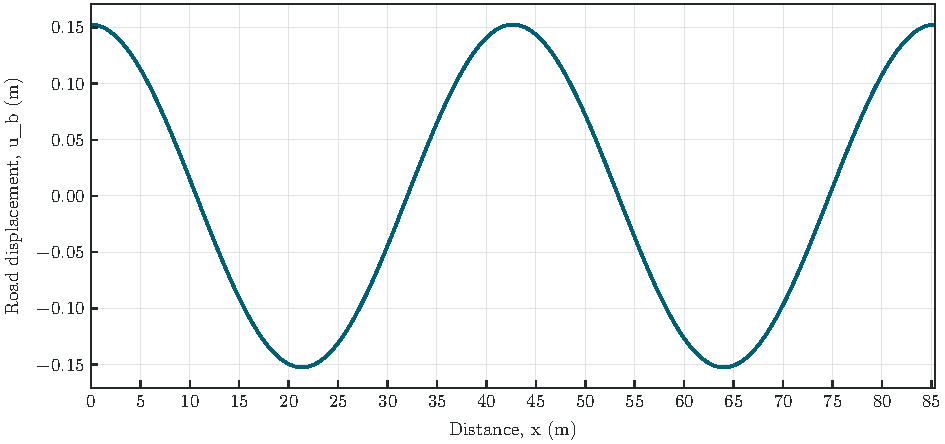
\includegraphics[width=0.90\linewidth]{figures/generated/solutions/A3-road.pdf}
\caption{A.3.3. Cosine road profile across two wavelengths.}
\end{figure}
\[\boxed{u_b(x)=0.1524\cos\!\left(\frac{2\pi x}{42.672\ \mathrm{m}}\right)\ \mathrm{m},\quad 0\leq x\leq85.344\ \mathrm{m}}\qquad\text{(A.3.3)}\]

\textbf{A.3.4. Road-frequency range.} At constant speed, $x=vt$ makes the road input $u_b(t)=a\cos(2\pi vt/\lambda)$, so $f=v/\lambda$. The maximum road frequency is therefore
\[
f_{\max}=\frac{v_{\max}}{\lambda}
=\frac{50.5155\ \mathrm{m/s}}{42.672\ \mathrm{m}}
=1.18381\ \mathrm{Hz}.
\]
I evaluate $f=\operatorname{linspace}(0,1.18381\ \mathrm{Hz},2000)$ for the plotted curves.
\[\boxed{f_{\max}=1.184\ \mathrm{Hz},\qquad N_f=2000}\qquad\text{(A.3.4)}\]

\textbf{A.3.5. Healthy-shock frequency response.} The figure plots the absolute body displacement transmissibility for healthy shocks. The matched-frequency marker is evaluated at exactly $f=f_n$, while the peak marker is evaluated at the analytic stationary point; neither marker is restricted to the sampled curve grid.
\begin{figure}[H]
\centering
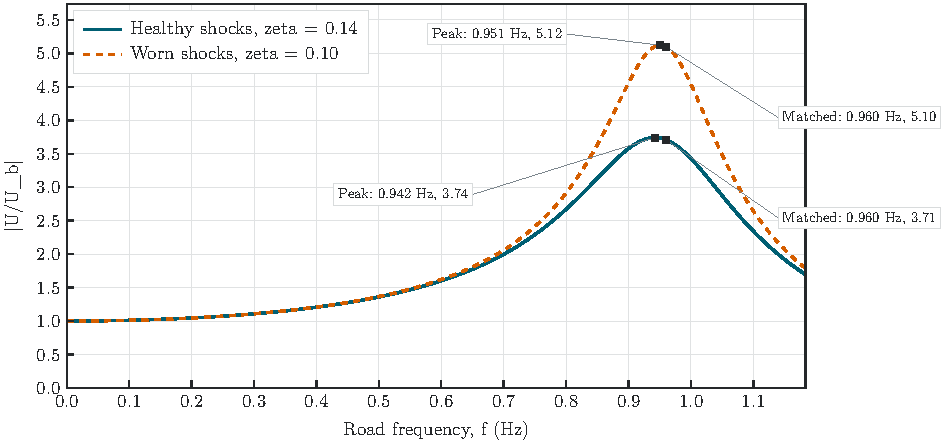
\includegraphics[width=0.94\linewidth]{figures/generated/solutions/A3-frequency.pdf}
\caption{A.3.5 and A.3.10. Absolute body-to-road displacement FRF versus road frequency. The curves compare healthy and worn shocks; square markers show analytic peak and matched-frequency events.}
\end{figure}

\textbf{A.3.6. Matched-frequency response.} At $r=1$, the complex response is $H(1)=1-i/(2\zeta)$, and its magnitude is
\[
|H_n|=\sqrt{1+\frac{1}{(2\zeta)^2}}
=\sqrt{1+\frac{1}{(0.280)^2}}=3.70879.
\]
The 2000-point sampled curve gives $|H|=3.70894$ at its nearest sample, while the analytic matched value is $3.70879$. For comparison, the true healthy maximum is $3.74053$ at $f=0.942367\ \mathrm{Hz}$, below $f_n$.
\[\boxed{\begin{aligned}
|H_n|&=3.71\quad\text{at }f=f_n=0.960\ \mathrm{Hz},\\
|H|_{\max}&=3.74\quad\text{at }f=0.942\ \mathrm{Hz}.
\end{aligned}}\qquad\text{(A.3.6)}\]

\textbf{A.3.7. Matched-frequency speed.} Since $f=v/\lambda$, setting $f=f_n$ gives
\[
v_n=f_n\lambda=(0.960\ \mathrm{Hz})(42.672\ \mathrm{m})
=40.9651\ \mathrm{m/s}=91.6364\ \mathrm{mph}.
\]
\[\boxed{v_n=41.0\ \mathrm{m/s}=91.6\ \mathrm{mph}}\qquad\text{(A.3.7)}\]

\textbf{A.3.8. Speed response and amplification limit.} The speed sweep uses 2000 equally spaced values from $0$ to $50.5155\ \mathrm{m/s}$, with $f=v/\lambda$. The analytic event values are reported separately from the sampled graph readings.
\begin{figure}[H]
\centering
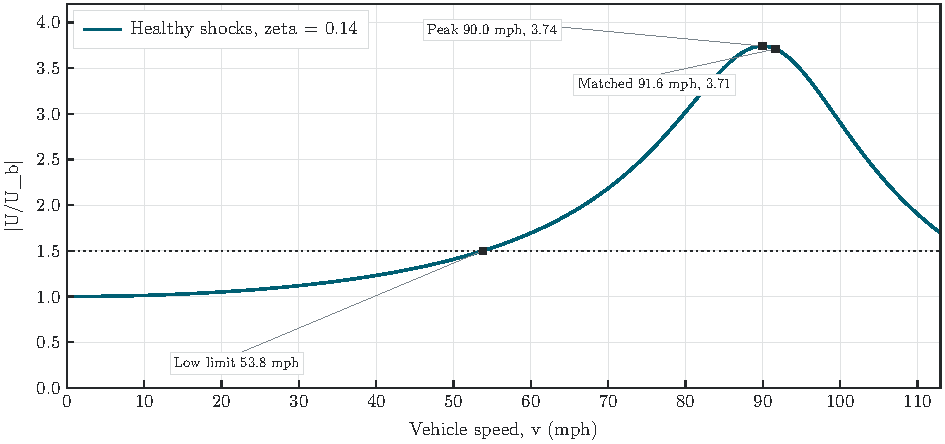
\includegraphics[width=0.94\linewidth]{figures/generated/solutions/A3-speed-healthy.pdf}
\caption{A.3.8. Healthy-shock absolute body-to-road displacement FRF versus vehicle speed. The dotted line is the 1.5 amplification threshold; square markers show analytic peak, matched-frequency, and in-range crossing events.}
\end{figure}
\begin{figure}[H]
\centering
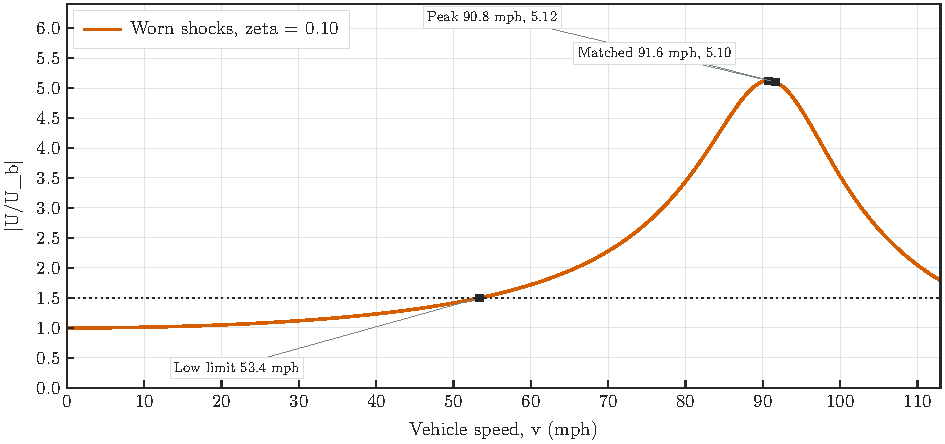
\includegraphics[width=0.94\linewidth]{figures/generated/solutions/A3-speed-worn.pdf}
\caption{A.3.10. Worn-shock absolute body-to-road displacement FRF versus vehicle speed. The dotted line is the 1.5 amplification threshold; square markers show analytic peak, matched-frequency, and in-range crossing events.}
\end{figure}

\textbf{(a) Matched-frequency event.} The speed conversion places $f_n$ at $v_n=91.6364\ \mathrm{mph}$, and the analytic ordinates are $|H_n|=3.70879$ for healthy shocks and $|H_n|=5.09902$ for worn shocks. These agree with A.3.6 and A.3.7.

\textbf{(b) True peak event.} Differentiating $|H|^2$ with respect to $q=r^2$ gives the stationary condition
\[
4\zeta^2q^2+2q-2=0.
\]
The positive root $q=[-1+\sqrt{1+8\zeta^2}]/(4\zeta^2)$ for $\zeta=0.140$ gives $r_{\mathrm{cr}}=\sqrt{q}=0.981632$, $f_{\mathrm{cr}}=0.942367\ \mathrm{Hz}$, $v_{\mathrm{cr}}=40.2127\ \mathrm{m/s}=89.9532\ \mathrm{mph}$, and $|H_{\max}|=3.74053$. This peak precedes the matched-frequency point. For worn shocks, $r_{\mathrm{cr}}=0.990334$, $f_{\mathrm{cr}}=0.950721\ \mathrm{Hz}$, $v_{\mathrm{cr}}=40.5692\ \mathrm{m/s}=90.7506\ \mathrm{mph}$, and $|H_{\max}|=5.12277$.

\textbf{(c) Threshold crossings.} Setting $q=r^2$ and $L=1.5$ reduces $|H|=L$ to
\[
L^2q^2+\bigl[L^2(4\zeta^2-2)-4\zeta^2\bigr]q+(L^2-1)=0.
\]
There are two positive crossings for each shock condition. The first crossing is the limit encountered when accelerating from rest; the second is the speed above which amplification falls below 1.5 again. The upper crossings lie above $v_{\max}$ and are not plotted.
\[
\boxed{\begin{aligned}
\zeta=0.140:&\quad v_{\mathrm{low}}=24.1\ \mathrm{m/s}=53.8\ \mathrm{mph},\\
&\quad v_{\mathrm{high}}=52.0\ \mathrm{m/s}=116.3\ \mathrm{mph},\\
\zeta=0.100:&\quad v_{\mathrm{low}}=23.9\ \mathrm{m/s}=53.4\ \mathrm{mph},\\
&\quad v_{\mathrm{high}}=52.4\ \mathrm{m/s}=117.3\ \mathrm{mph}.
\end{aligned}}\qquad\text{(A.3.8)}\]

\textbf{A.3.9. Wavelength for a 30 mph critical speed.} The requested speed is the true peak speed, not the matched-frequency speed. Using the healthy-shock peak frequency $f_{\mathrm{cr}}=0.942367\ \mathrm{Hz}$, choose
\[
\lambda_{\mathrm{new}}=\frac{v_{\mathrm{cr,target}}}{f_{\mathrm{cr}}}
=\frac{13.4112\ \mathrm{m/s}}{0.942367\ \mathrm{Hz}}
=14.2314\ \mathrm{m}.
\]
\[\boxed{\lambda_{\mathrm{new}}=14.23\ \mathrm{m}=46.7\ \mathrm{ft}}\qquad\text{(A.3.9)}\]

\textbf{A.3.10. Worn shocks.} Repeating items (5)--(8) with $\zeta=0.100$ retains the same matched frequency $f_n=0.960\ \mathrm{Hz}$ and matched speed $v_n=91.6364\ \mathrm{mph}$, but increases the matched response to
\[
|H_n|=\sqrt{1+\frac{1}{(0.200)^2}}=5.09902.
\]
The true peak is $|H|_{\max}=5.12277$ at $f_{\mathrm{cr}}=0.950721\ \mathrm{Hz}$ and $v_{\mathrm{cr}}=40.5692\ \mathrm{m/s}=90.7506\ \mathrm{mph}$. The table compares both shock conditions. Since $|H|^2$ increases with damping ratio for $r>\sqrt{2}$, the healthy response exceeds the worn response at high frequency, even though lower damping produces a much larger resonance peak.
{\begin{center}\small\begin{tabular}{@{}lrrrr@{}}
\toprule\noalign{}
Shock condition & $|H_n|$ & $f_{\mathrm{cr}}$ (Hz) & Peak $|H|$ & $v_{\mathrm{cr}}$ (mph) \\
\midrule\noalign{}
Healthy, $\zeta=0.140$ & 3.71 & 0.942 & 3.74 & 90.0 \\
Worn, $\zeta=0.100$ & 5.10 & 0.951 & 5.12 & 90.8 \\
\bottomrule\end{tabular}\end{center}}

\[\boxed{|H_n|_{\mathrm{worn}}=5.10,\quad |H|_{\max,\mathrm{worn}}=5.12\text{ at }0.951\ \mathrm{Hz}}\qquad\text{(A.3.10)}\]

\noindent\begin{minipage}{\linewidth}\color{black}
\textbf{Graph readings.} MATLAB data tips on the 2000-point sampled curves give the readings below. The speed-grid spacing is $0.0565\,\mathrm{mph}$, so sampled extrema and threshold values differ slightly from the analytic events above.
\begin{center}\small
\begin{tabular}{@{}lrrrr@{}}
\toprule
Event & Healthy $x$ & Healthy $|H|$ & Worn $x$ & Worn $|H|$ \\
\midrule
Peak frequency (Hz) & 0.942 & 3.74 & 0.950 & 5.12 \\
Matched frequency (Hz) & 0.960 & 3.71 & 0.960 & 5.10 \\
Peak speed (mph) & 89.9 & 3.74 & 90.7 & 5.12 \\
Matched speed (mph) & 91.6 & 3.71 & 91.6 & 5.10 \\
Lower crossing (mph) & 53.8 & 1.500 & 53.4 & 1.500 \\
Upper crossing & outside sweep & -- & outside sweep & -- \\
\bottomrule
\end{tabular}
\end{center}
\end{minipage}\par
\clearpage
\matlabcaption{MATLAB calculations and direct plots for A.3.}
\lstinputlisting[style=hwmatlab]{matlab/A3.m}

\clearpage
\subsection{A.4 Standing Waves}
\questionitem{1}{Nothing here}
\questionitem{2}{Nothing here}
\questionitem{3}{Assume wavespeed \ensuremath{c=340\,\mathrm{m}/\mathrm{s}} and frequency \ensuremath{f=3.6\,\mathrm{kHz}}. Calculate:}
\subquestionitem{a}{Rad/sec frequency \ensuremath{\omega}}
\subquestionitem{b}{Wavenumber \ensuremath{\gamma}}
\subquestionitem{c}{Wavelength \ensuremath{\lambda}}
\subquestionitem{d}{Distance \ensuremath{\Delta x} between standing wave nodes}
\questionitem{4}{Nothing here}

\clearpage
\subsection*{Solution to A.4}
\textbf{3. Input data.} The specified wavespeed and frequency are
\[
\boxed{c=340\,\mathrm{m/s},\qquad f=3.6\,\mathrm{kHz}=3600\,\mathrm{Hz}.}
\]
Using the standing-wave relations from HW02 and the course notes (pp.~75--77),
\[
\omega=2\pi f,\qquad \gamma=\frac{\omega}{c},\qquad
\lambda=\frac{c}{f},\qquad \Delta x=\frac{\lambda}{2}.
\]
The angular frequency is
\[
\omega=2\pi(3600)=22619.5\,\mathrm{rad/s}
\quad\Longrightarrow\quad
\boxed{\omega=2.26\times10^4\,\mathrm{rad/s}.}\qquad\text{(A.4.3.a)}
\]
The corresponding wavenumber is
\[
\gamma=\frac{22619.5}{340}=66.5278\,\mathrm{rad/m}
\quad\Longrightarrow\quad
\boxed{\gamma=66.5\,\mathrm{rad/m}.}\qquad\text{(A.4.3.b)}
\]
The wavelength is
\[
\lambda=\frac{340}{3600}\,\mathrm{m}=0.0944444\,\mathrm{m}
\quad\Longrightarrow\quad
\boxed{\lambda=94.4\,\mathrm{mm}.}\qquad\text{(A.4.3.c)}
\]
Adjacent standing-wave nodes are separated by half a wavelength, so
\[
\Delta x=\frac{0.0944444}{2}\,\mathrm{m}
\quad\Longrightarrow\quad
\boxed{\Delta x=47.2\,\mathrm{mm}.}\qquad\text{(A.4.3.d)}
\]

\clearpage
\matlabcaption{MATLAB calculations for A.4.3.}
\lstinputlisting[style=hwmatlab]{matlab/A4.m}

\clearpage
\subsection{A.5 Musical Notes}
\questionitem{1}{Find the Hz frequency of note \ensuremath{E_{4}}}
\questionitem{2}{Find what musical note corresponds to \ensuremath{1396.9\,\mathrm{Hz}}}
\questionitem{3}{What is the commonly accepted frequency range of human hearing?}
\questionitem{4}{What is the lowest frequency on the scale of equal temperament and what musical note does it correspond to?}
\questionitem{5}{What is the highest frequency on the scale of equal temperament and what musical note does it correspond to?}
\questionitem{6}{Graduate work. Explain the scale of equal temperament by answering items (a)--(c)}
\subquestionitem{a}{What is the organizing principle of the scale of equal temperament}
\subquestionitem{b}{How many equal-temperament entries are in an octave?}
\subquestionitem{c}{What is the ratio between two adjacent entries on the scale of equal temperament?}
\clearpage
\subsection*{Solution to A.5}
The course notes anchor the equal-temperament scale at $A_4=440\ \mathrm{Hz}$ and divide each octave into twelve equal semitone intervals. If $n$ is the number of semitones above or below $A_4$, the frequency is
\[
f_n=440\,2^{n/12}\ \mathrm{Hz}.
\]
The input values and the note range shown in the course-note chart are
\begin{center}\small
\begin{tabular}{@{}lrl@{}}
\toprule\noalign{}
Quantity & Value & Unit \\
\midrule\noalign{}
$A_4$ & 440 & Hz \\
$f$ & 1396.9 & Hz \\
Chart range & $C_0$--$C_{10}$ & notes \\
\bottomrule
\end{tabular}
\end{center}
The chart appears on page 90 of the course notes.

For A.5.1, $E_4$ is five semitones below $A_4$. For A.5.2, the frequency-to-note relation gives the semitone offset
\[
n=12\log_2\!\left(\frac{1396.9}{440}\right)=19.9998\approx20,
\]
so the supplied frequency corresponds to $F_6$, twenty semitones above $A_4$.
\[
\begin{aligned}
f_{E_4}&=440\,2^{-5/12}=329.627557\ \mathrm{Hz}\approx\boxed{330\ \mathrm{Hz}} &&\text{(A.5.1)},\\
f_{F_6}&=440\,2^{20/12}=1396.912926\ \mathrm{Hz}\approx1396.9\ \mathrm{Hz},\\
1396.9\ \mathrm{Hz}&\longleftrightarrow\boxed{F_6} &&\text{(A.5.2)}.
\end{aligned}
\]

The commonly accepted hearing range is approximately $20\ \mathrm{Hz}$ to $20\ \mathrm{kHz}$.
\[
\boxed{20\ \mathrm{Hz}\leq f\leq20\ \mathrm{kHz}}\qquad\text{(A.5.3)}
\]

To compare the musical scale with this hearing range, the course-note chart begins at $C_0$ and ends at $C_{10}$. Applying the same equation gives its endpoints. Equal temperament itself continues by octave in both directions, so the mathematical scale has no absolute lowest or highest frequency.
\[
\begin{aligned}
f_{C_0}&=440\,2^{-57/12}=16.351598\ \mathrm{Hz}\approx\boxed{16.35\ \mathrm{Hz}\text{ at }C_0} &&\text{(A.5.4, chart minimum)},\\
f_{C_{10}}&=440\,2^{63/12}=16744.036179\ \mathrm{Hz}\approx\boxed{16.74\ \mathrm{kHz}\text{ at }C_{10}} &&\text{(A.5.5, chart maximum)}.
\end{aligned}
\]

Equal temperament spaces the twelve semitone steps uniformly on a logarithmic frequency scale. Each successive entry is therefore the previous frequency multiplied by the same factor, and twelve such steps double the frequency to reach the same note in the next octave.
\[
\boxed{\begin{aligned}
\text{entries per octave}&=12,\\
\frac{f_{n+1}}{f_n}&=2^{1/12}\approx1.059,\\
\left(2^{1/12}\right)^{12}&=2.
\end{aligned}}\qquad\text{(A.5.6)}
\]

\clearpage
\matlabcaption{MATLAB calculations for A.5.}
\lstinputlisting[style=hwmatlab]{matlab/A5.m}

\clearpage
\section{Fluid Waves and Vibration}
\subsection{B.4 Calculate Air Vibration in a Tube Closed at Both Ends}
Consider a tube of length \ensuremath{L=0.50\,\mathrm{m}} closed at both ends. Take sound speed \ensuremath{c=340\,\mathrm{m}/\mathrm{s}} and air density \ensuremath{\rho=1.2\,\mathrm{kg}/\mathrm{m}^{3}}. Use the results of Problem B.3 to calculate the modal vibration characteristics and modeshapes for \ensuremath{j=1,\ldots,N} with \ensuremath{N=5}.\par
\questionitem{1}{Display input data}
\questionitem{2}{Calculate and display the modal vibration characteristics:}
\subquestionitem{a}{Eigenvalues \ensuremath{z_{j}}}
\subquestionitem{b}{Wavenumbers \ensuremath{\gamma_{j}}}
\subquestionitem{c}{Rad/s frequencies \ensuremath{\omega_{j}}}
\subquestionitem{d}{Hz frequencies \ensuremath{f_{j}}}
\questionitem{3}{Calculate and plot the displacement modeshapes}
\questionitem{4}{Discuss your results}
\questionitem{5}{Graduate work. Calculate and plot the normalized pressure modeshapes, and compare the result with item (3)}
\clearpage
\subsection*{Solution to B.4}
\textbf{1. Input data.} The physical parameters specified for the closed-closed acoustic tube are
\[
\boxed{L=0.500\,\mathrm{m},\qquad c=340\,\mathrm{m/s},\qquad \rho=1.2\,\mathrm{kg/m}^3,\qquad N=5}\qquad\text{(B.4.1)}
\]
The associated medium properties are the acoustic bulk modulus and the characteristic acoustic impedance.
\[
K=\rho c^2=1.2\times(340)^2\,\mathrm{Pa}\approx138.7\,\mathrm{kPa},
\qquad
Z=\rho c=1.2\times 340\,\mathrm{Pa\cdot s/m}=408\,\mathrm{rayl}.
\]

\textbf{2. Modal vibration characteristics.} Using the analytical relations derived in Problem B.3, the modal characteristics for modes $j=1,2,3,4,5$ are evaluated as follows:
\par\smallskip\noindent
\textbf{(a) Eigenvalues $z_j$:}
\[
\boxed{z_j=j\pi\quad\Longrightarrow\quad z_1=\pi,\; z_2=2\pi,\; z_3=3\pi,\; z_4=4\pi,\; z_5=5\pi}\qquad\text{(B.4.2.a)}
\]
\textbf{(b) Wavenumbers $\gamma_j$:}
\[
\boxed{\gamma_j=\frac{z_j}{L}=\frac{j\pi}{0.500}\,\mathrm{rad/m}\approx 6.28\,j\,\mathrm{rad/m}}\qquad\text{(B.4.2.b)}
\]
\textbf{(c) Natural circular frequencies $\omega_j$:} Since $c/L=340/0.500=680\,\mathrm{s}^{-1}$,
\[
\boxed{\omega_j=\gamma_j c=\frac{j\pi c}{L}=680\pi j\,\mathrm{rad/s}\approx 2.14\times10^3\,j\,\mathrm{rad/s}}\qquad\text{(B.4.2.c)}
\]
\textbf{(d) Natural frequencies $f_j$ in Hz:}
\[
\boxed{f_j=\frac{\omega_j}{2\pi}=\frac{jc}{2L}=340\,j\,\mathrm{Hz}\quad\Longrightarrow\quad 340,\,680,\,1020,\,1360,\,1700\,\mathrm{Hz}}\qquad\text{(B.4.2.d)}
\]
The corresponding acoustic wavelengths are $\lambda_j=2L/j=1.000/j\,\mathrm{m}$. The complete modal characteristics are summarized in Table~\ref{tab:hw02-b4-modal}.

\begin{table}[H]
\centering
\caption{Modal vibration characteristics of the closed-closed air tube ($L=0.500\,\mathrm{m}$, $c=340\,\mathrm{m/s}$).}
\label{tab:hw02-b4-modal}
\smallskip
\small
\begin{tabular}{@{}cccccc@{}}
\toprule
Mode $j$ & $z_j$ (rad) & $\gamma_j$ (rad/m) & $\omega_j$ (krad/s) & $f_j$ (Hz) & $\lambda_j$ (m) \\
\midrule
1 & $\pi\approx 3.14$ & $6.28$ & $2.14$ & $340$ & $1.000$ \\
2 & $2\pi\approx 6.28$ & $12.57$ & $4.27$ & $680$ & $0.500$ \\
3 & $3\pi\approx 9.42$ & $18.85$ & $6.41$ & $1020$ & $0.333$ \\
4 & $4\pi\approx 12.57$ & $25.1$ & $8.55$ & $1360$ & $0.250$ \\
5 & $5\pi\approx 15.71$ & $31.4$ & $10.68$ & $1700$ & $0.200$ \\
\bottomrule
\end{tabular}
\end{table}

\textbf{3. Displacement modeshapes.} From Problem B.3 (item 20), the displacement modeshapes are
\[
\boxed{U_j(x)=\sin\left(\frac{j\pi x}{L}\right)=\sin\left(\frac{j\pi x}{0.500}\right),\qquad j=1,\ldots,5}\qquad\text{(B.4.3)}
\]
Figure~\ref{fig:hw02-b4-disp} plots the displacement modeshapes for the first five modes across the tube length.

\begin{figure}[H]
\centering
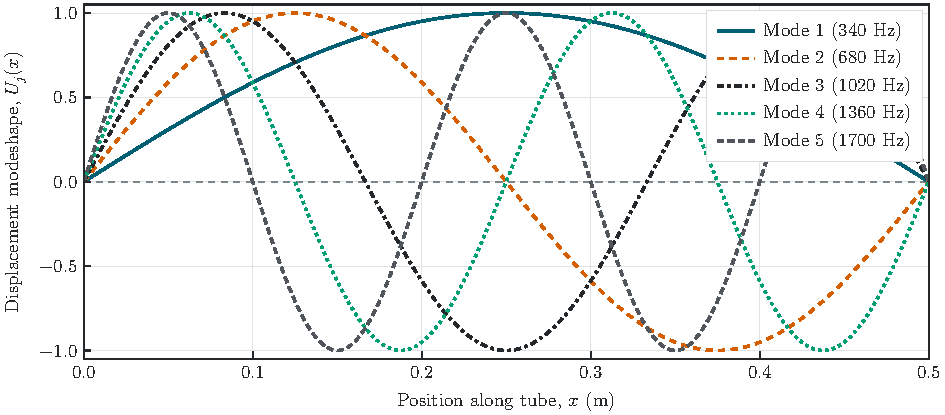
\includegraphics[width=0.96\linewidth]{figures/generated/solutions/B4-displacement.pdf}
\caption{Displacement modeshapes $U_j(x)=\sin(j\pi x/L)$ for modes $j=1,\ldots,5$ in an air tube of length $L=0.500\,\mathrm{m}$ closed at both ends. }
\label{fig:hw02-b4-disp}
\end{figure}

\textbf{4. Discussion of results.}
Both rigid ends are displacement nodes because $U_j(0)=U_j(L)=0$. The fundamental is $f_1=340\,\mathrm{Hz}$, and the higher frequencies are $f_j=jf_1$. The tube therefore supports all integer harmonics.

Each mode fits $j$ half-wavelengths into the tube, so $L=j\lambda_j/2$. For the fundamental, $\lambda_1=2L=1.000\,\mathrm{m}$. Mode $j$ has $j+1$ displacement nodes, including both ends, and $j$ antinodes. Adjacent nodes are separated by $L/j$.


\textbf{5. Graduate work: Normalized pressure modeshapes and comparison.}
From Problem B.3 (item 21), acoustic pressure disturbance is generated by fluid strain, $p(x,t)=-Ku_x(x,t)=-\rho c^2 u_x(x,t)$. For displacement amplitude $a_j>0$ in meters, write $u_j(x,t)=a_jU_j(x)e^{-i\omega_jt}$. Differentiating $U_j(x)=\sin(\gamma_jx)$ gives $U_j'(x)=\gamma_j\cos(\gamma_j x)$, yielding the pressure amplitude
\[
P_j(x)=-\rho c^2a_j\gamma_j\cos\left(\frac{j\pi x}{L}\right)=-\rho c\,\omega_j a_j\cos\left(\frac{j\pi x}{L}\right).
\]
\noindent\begin{minipage}{\linewidth}\color{black}
Normalizing by the peak pressure amplitude $|P_j|_{\max}=\rho c\,\omega_j a_j$ yields the normalized pressure modeshape
\[
\boxed{\bar{P}_j(x)=-\cos\left(\frac{j\pi x}{L}\right)=-\cos\left(\frac{j\pi x}{0.500}\right),\qquad j=1,\ldots,5}\qquad\text{(B.4.5)}
\]
\end{minipage}\par

Figure~\ref{fig:hw02-b4-press} plots the normalized pressure modeshapes for modes $1$ through $5$.

\begin{figure}[H]
\centering
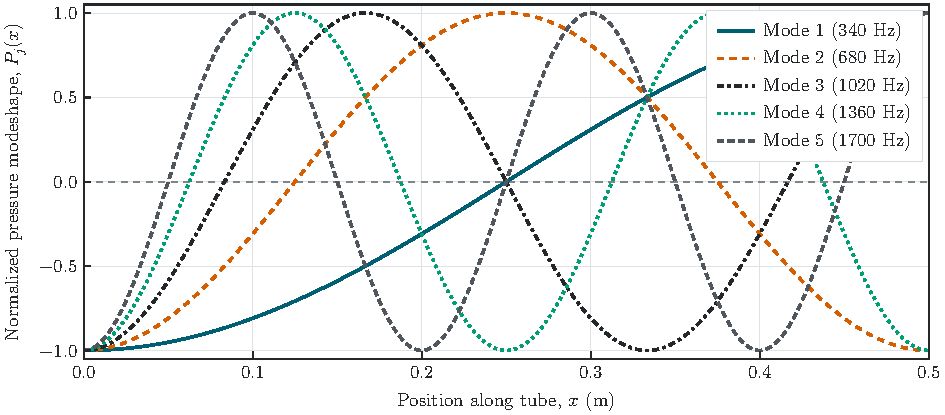
\includegraphics[width=0.96\linewidth]{figures/generated/solutions/B4-pressure.pdf}
\caption{Normalized acoustic pressure modeshapes $\bar{P}_j(x)=-\cos(j\pi x/L)$ for modes $j=1,\ldots,5$ in a closed-closed tube of length $L=0.500\,\mathrm{m}$.}
\label{fig:hw02-b4-press}
\end{figure}

The sine displacement shape and negative-cosine pressure shape differ spatially by a quarter wavelength. Since pressure is proportional to $-U_j'$, displacement antinodes are pressure nodes, and displacement nodes are pressure antinodes.

Both closed ends are pressure antinodes with $|\bar{P}_j|=1$. Mode $j$ has $j$ internal pressure nodes and $j+1$ pressure antinodes, including the two ends. These counts agree with the plotted curves.

\clearpage
\matlabcaption{MATLAB calculations and plots for B.4.}

\lstinputlisting[style=hwmatlab]{matlab/B4.m}

\clearpage
\subsection{B.5 Calculate the Slide Whistle}
Consider the slide whistle shown in Figure~\ref{fig:test02-whistle}. Take $c=340\,\mathrm{m/s}$, residual cavity length $L_0=10\,\mathrm{mm}$, fully extended length $L_e=420\,\mathrm{mm}$, and fully contracted length $L_c=260\,\mathrm{mm}$. Calculate the fundamental frequency for various slider positions.
\begin{figure}[H]
\centering
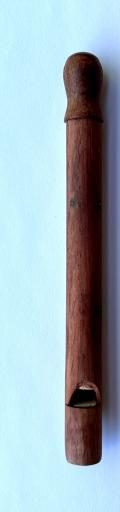
\includegraphics[angle=270,width=0.55\linewidth]{figures/original/test2-001.jpg}\par
{\small (a)}\par\smallskip
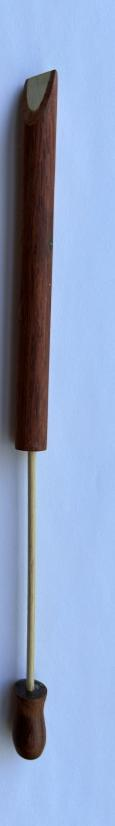
\includegraphics[angle=90,width=0.85\linewidth]{figures/original/test2-002.jpg}\par
{\small (b)}
\caption{Slide whistle. (a) Fully retracted, showing the piston tip and residual cavity. (b) Fully extended.}
\label{fig:test02-whistle}
\end{figure}
\taskprompt
\questionitem{1}{Display input data $c$ and $L_0$}
\questionitem{2}{Display the supplied fully extended whistle length \ensuremath{L_{e}}}
\questionitem{3}{Display the supplied fully contracted whistle length \ensuremath{L_{c}}}
\questionitem{4}{Use \ensuremath{L_{e}}, \ensuremath{L_{c}} to calculate the extension travel \ensuremath{dL_{I}} corresponding to fully extended slide whistle}
\questionitem{5}{Use \ensuremath{dL_{I}} and \ensuremath{L_{0}} to calculate the cavity length \ensuremath{L_{I}} of a fully extended slide whistle}
\questionitem{6}{Estimate the fully extended frequency \ensuremath{f_{I}} in Hz and find the nearest musical note expressed as a letter name and octave number (e.g., \ensuremath{\mathrm{G3}} signifies note G in the third octave)}
\questionitem{7}{Use \ensuremath{L_{e}}, \ensuremath{L_{c}} to calculate the extension travel \ensuremath{dL_{\mathrm{II}}} corresponding to \ensuremath{50\%} extended slide whistle}
\questionitem{8}{Use \ensuremath{dL_{\mathrm{II}}} and \ensuremath{L_{0}} to calculate the cavity length \ensuremath{L_{\mathrm{II}}} of a \ensuremath{50\%}-extended slide whistle}
\questionitem{9}{Calculate the \ensuremath{50\%}-extended frequency \ensuremath{f_{\mathrm{II}}} in Hz and find the nearest musical note expressed as a letter name and an octave number}
\questionitem{10}{Comment on your work}
\subsubsection*{Graduate Work}
Estimate the piston position required to obtain the musical note \ensuremath{\mathrm{D7}}.

\taskprompt
\questionitem{11}{Display the frequency \ensuremath{f_{\mathrm{III}}} of the note \ensuremath{\mathrm{D7}}}
\questionitem{12}{Calculate the cavity length \ensuremath{L_{\mathrm{III}}} needed to generate frequency \ensuremath{f_{\mathrm{III}}} of the note \ensuremath{\mathrm{D7}}}
\questionitem{13}{Calculate the extension travel \ensuremath{dL_{\mathrm{III}}} needed to generate frequency \ensuremath{f_{\mathrm{III}}} of the note \ensuremath{\mathrm{D7}}}
\questionitem{14}{Estimate what percentage of the piston must be extended to generate the note \ensuremath{\mathrm{D7}}}
\questionitem{15}{Comment on your work}
\clearpage
\subsection*{Solution to B.5}
\textbf{1. Input data.} The specified dimensions and sound speed are
\[
\boxed{\begin{aligned}
L_{0}&=10.0\,\mathrm{mm}=0.0100\,\mathrm{m},&
c&=340\,\mathrm{m/s},\\
L_{e}&=420\,\mathrm{mm}=0.420\,\mathrm{m},&
L_{c}&=260\,\mathrm{mm}=0.260\,\mathrm{m}.
\end{aligned}}
\]
The supplied Figure~\ref{fig:test02-whistle} identifies the instrument configuration. The main calculation uses the closed--closed idealization developed in the course notes on pp.~109--113. Those notes allow a small opening for the sound to escape while retaining closed displacement conditions at both ends. The supplied lengths are used directly, so no ruler digitization is required.

\textbf{2. Fully extended whistle length.} The supplied fully extended length is
\[
\boxed{L_{e}=0.420\,\mathrm{m}.}
\]

\textbf{3. Fully contracted whistle length.} The supplied fully contracted length is
\[
\boxed{L_{c}=0.260\,\mathrm{m}.}
\]

\textbf{4. Fully extended travel.} The extension travel is the difference between the two specified overall lengths,
\[
\boxed{dL_{\mathrm{I}}=L_{e}-L_{c}=0.420-0.260=0.1600\,\mathrm{m}.}
\]

\textbf{5. Fully extended cavity length.} Adding the residual cavity to the travel gives
\[
\boxed{L_{\mathrm{I}}=L_{0}+dL_{\mathrm{I}}=0.0100+0.1600=0.1700\,\mathrm{m}.}
\]

\textbf{6. Fully extended frequency.} For the adopted closed--closed idealization, the fundamental frequency from the course notes is
\[
f=\frac{c}{2L}.
\]
Therefore,
\[
f_{\mathrm{I}}=\frac{340}{2(0.170)}=1.000\times10^{3}\,\mathrm{Hz}.
\]
The nearest equal-tempered note is
\[
\boxed{f_{\mathrm{I}}=1.000\,\mathrm{kHz},\qquad \text{nearest note }\mathrm{B5}\ (988\,\mathrm{Hz}).}
\]

\textbf{7. Fifty-percent extension travel.} The travel at the specified half-extension is
\[
\boxed{dL_{\mathrm{II}}=0.50dL_{\mathrm{I}}=0.50(0.160)=0.0800\,\mathrm{m}.}
\]

\textbf{8. Fifty-percent extension cavity length.} Adding the residual cavity gives
\[
\boxed{L_{\mathrm{II}}=L_{0}+dL_{\mathrm{II}}=0.0100+0.0800=0.0900\,\mathrm{m}.}
\]

\textbf{9. Fifty-percent extension frequency.} The closed--closed fundamental is
\[
f_{\mathrm{II}}=\frac{340}{2(0.0900)}=1.889\times10^{3}\,\mathrm{Hz}.
\]
The nearest equal-tempered note is
\[
\boxed{f_{\mathrm{II}}=1.889\,\mathrm{kHz},\qquad \text{nearest note }\mathrm{A\sharp6}\ (1.865\,\mathrm{kHz}).}
\]

\textbf{10. Comment.} Increasing the cavity length lowers the fundamental frequency because the closed--closed relation is inversely proportional to \(L\). The half-extended cavity is shorter than the fully extended cavity, so its frequency is higher, as the two calculated values show. The closed--closed model is the main course-note idealization used here; the Test 2 prompt does not explicitly direct the reader to recall Problem B.3.

\textbf{11. Frequency of D7.} Using equal temperament with the standard \(440\,\mathrm{Hz}\) A4 reference,
\[
\boxed{f_{\mathrm{III}}=440\,2^{29/12}=2.35\times10^{3}\,\mathrm{Hz}.}
\]

\textbf{12. Cavity length for D7.} Applying the closed--closed fundamental relation gives
\[
\boxed{L_{\mathrm{III}}=\frac{c}{2f_{\mathrm{III}}}
=\frac{340}{2(2349.318)}=0.0724\,\mathrm{m}.}
\]

\textbf{13. Extension travel for D7.} The required travel beyond the residual cavity is
\[
\boxed{dL_{\mathrm{III}}=L_{\mathrm{III}}-L_{0}=0.0724-0.0100=0.0624\,\mathrm{m}.}
\]

\textbf{14. Required piston extension.} Relative to the full available travel,
\[
\boxed{100\frac{dL_{\mathrm{III}}}{dL_{\mathrm{I}}}
=100\frac{0.0624}{0.160}=39.0\%.}
\]

\textbf{15. Comment.} The D7 target requires approximately \(39.0\%\) of the available piston travel under the main closed--closed model, so it lies within the specified \(0\)--\(100\%\) range. Figure~\ref{fig:test02-whistle} shows a physical open fipple and a closed piston, which motivates the alternative closed--open model from the course notes on pp.~114--117. Under that model, \(f=c/(4L)\), giving \(5.00\times10^{2}\,\mathrm{Hz}\) at full extension, nearest B4, \(944\,\mathrm{Hz}\) at 50\% extension, nearest \(\mathrm{A\sharp5}\), and a D7 position of \(L_{\mathrm{III}}=36.2\,\mathrm{mm}\), \(dL_{\mathrm{III}}=26.2\,\mathrm{mm}\), or \(16.4\%\) travel. Both boundary models produce a feasible D7 position; the closed--closed values above are the primary course-note idealization.

\clearpage
\matlabcaption{MATLAB calculations for B.5.}
\lstinputlisting[style=hwmatlab]{matlab/B5.m}

\clearpage
\subsection{B.6 Calculate Sound Intensity and the dB Scale}
Take sound speed \ensuremath{c=340\,\mathrm{m}/\mathrm{s}} and air density \ensuremath{\rho=1.2\,\mathrm{kg}/\mathrm{m}^{3}}.

\taskprompt
\questionitem{1}{Display input data}
\questionitem{2}{Calculate air’s acoustic impedance \ensuremath{Z}}
\questionitem{3}{Calculate the sound intensity \ensuremath{I} corresponding to a sound pressure \ensuremath{p=88\,\mathrm{mPa}}}
\questionitem{4}{Give the values of the reference sound intensity \ensuremath{I_{0}} and reference sound pressure \ensuremath{p_{0}}}
\questionitem{5}{Convert the sound pressure and sound intensity from item (3) to decibels}
\questionitem{6}{Verify that the sound pressure and sound intensity calculated at item (5) have the same dB value and explain why it is so}
\questionitem{7}{Calculate in physical units the sound intensity, sound pressure, and sound power from a loudspeaker with diameter \ensuremath{D=1.25\,\mathrm{m}} working at \ensuremath{72\,\mathrm{dB}}}
\questionitem{8}{Calculate the sound pressure \ensuremath{p_{\mathrm{horn}}} created by a \ensuremath{124\,\mathrm{dB}} car horn}
\questionitem{9}{Give the values of the pain sound intensity \ensuremath{I_{\mathrm{pain}}} and pain sound pressure \ensuremath{p_{\mathrm{pain}}} and comment on the results of items (7) and (8) relative to pain values}
\questionitem{10}{Graduate work. Explain why different decibel-conversion formulas are required for sound intensity \ensuremath{I} and sound pressure \ensuremath{p}}
\clearpage
\subsection*{Solution to B.6}
\begingroup
\setlength{\abovedisplayskip}{6pt}
\setlength{\belowdisplayskip}{6pt}
\setlength{\abovedisplayshortskip}{4pt}
\setlength{\belowdisplayshortskip}{4pt}
\setlength{\intextsep}{6pt}

\textbf{1. Input data.} The specified sound speed and air density are
\[
\boxed{c=340\,\mathrm{m/s},\qquad \rho=1.2\,\mathrm{kg/m^3}.}
\]
The specified pressure, loudspeaker diameter, and sound levels are
\[
\boxed{p=88\,\mathrm{mPa}=0.088\,\mathrm{Pa},\qquad
D=1.25\,\mathrm{m},\qquad L_{\mathrm{sp}}=72\,\mathrm{dB},\qquad
L_{\mathrm{horn}}=124\,\mathrm{dB}.}
\]

\textbf{2. Acoustic impedance.} The plane-wave acoustic impedance is
\[
Z=\rho c=(1.2)(340)=\boxed{408\,\mathrm{rayl}.}
\]

\textbf{3. Sound intensity for $p=88\,\mathrm{mPa}$.} Following the course-note convention,
\[
I=\frac{p^2}{Z}=\frac{(0.088)^2}{408}
  =\boxed{1.898\times10^{-5}\,\mathrm{W/m^2}}.
\]

\textbf{4. Reference intensity and pressure.} The reference intensity is
\[
\boxed{I_0=10^{-12}\,\mathrm{W/m^2}=1\,\mathrm{pW/m^2}.}
\]
Using the specified $Z$ without rounding,
\[
p_0=\sqrt{ZI_0}=\sqrt{(408)(10^{-12})}
 \approx\boxed{20.2\,\mu\mathrm{Pa}}.
\]

\textbf{5. Decibel values for the specified pressure.} The intensity and pressure levels are
\[
L_I=10\log_{10}\left(\frac{I}{I_0}\right)=72.8\,\mathrm{dB},
\qquad
L_p=20\log_{10}\left(\frac{p}{p_0}\right)=72.8\,\mathrm{dB}.
\]
Therefore,
\[
\boxed{L_I=L_p=72.8\,\mathrm{dB}.}
\]

\textbf{6. Equality of the two decibel values.} Since $I=p^2/Z$ and $I_0=p_0^2/Z$,
\[
\frac{I}{I_0}=\left(\frac{p}{p_0}\right)^2,
\qquad
10\log_{10}\left(\frac{I}{I_0}\right)=20\log_{10}\left(\frac{p}{p_0}\right).
\]
The two levels therefore agree when the reference pressure satisfies $p_0^2=ZI_0$.

\textbf{7. Loudspeaker at $72\,\mathrm{dB}$.} The intensity corresponding to the loudspeaker level is
\[
I_{\mathrm{sp}}=I_0 10^{L_{\mathrm{sp}}/10}
 =\boxed{15.85\,\mu\mathrm{W/m^2}}.
\]
The corresponding pressure and circular-face area are
\[
p_{\mathrm{sp}}=\sqrt{ZI_{\mathrm{sp}}}=\boxed{80.4\,\mathrm{mPa}},
\qquad
A=\frac{\pi D^2}{4}=1.23\,\mathrm{m^2}.
\]
Assuming the stated intensity is uniform over that area, the sound power is
\[
P_{\mathrm{sp}}=I_{\mathrm{sp}}A=\boxed{19.45\,\mu\mathrm{W}}.
\]

\textbf{8. Pressure from a $124\,\mathrm{dB}$ car horn.} The horn pressure is
\[
p_{\mathrm{horn}}=p_0 10^{L_{\mathrm{horn}}/20}
 =\boxed{32.0\,\mathrm{Pa}}.
\]
For comparison, the corresponding intensity is $I_{\mathrm{horn}}=2.51\,\mathrm{W/m^2}$.

\textbf{9. Pain-threshold comparison.} The course-note pain references are
\[
\boxed{I_{\mathrm{pain}}=1\,\mathrm{W/m^2},\qquad
p_{\mathrm{pain}}=\sqrt{ZI_{\mathrm{pain}}}=20.2\,\mathrm{Pa}.}
\]
The pain level is $120\,\mathrm{dB}$. The loudspeaker is $48\,\mathrm{dB}$ below this level, with intensity ratio $1.585\times10^{-5}$ and pressure ratio $3.981\times10^{-3}$. The horn is $4\,\mathrm{dB}$ above the pain level, with intensity ratio $2.51$ and pressure ratio $1.585$; its pressure is therefore $32.0\,\mathrm{Pa}$, above the $20.2\,\mathrm{Pa}$ pain reference.

\textbf{10. Graduate work.} Intensity is proportional to pressure squared at fixed acoustic impedance. The intensity level therefore uses $10\log_{10}$, while the pressure level uses $20\log_{10}$,
\[
10\log_{10}\left(\frac{I}{I_0}\right)
=20\log_{10}\left(\frac{p}{p_0}\right).
\]

\clearpage
\matlabcaption{MATLAB calculations for B.6.}
\lstinputlisting[style=hwmatlab]{matlab/B6.m}
\endgroup

\clearpage
\section{Extra Credit Challenge Problems}
Challenge problems are optional.\par
\subsection{C.3 Calculate Air Vibration in a Tube with Various Boundary Conditions}
Consider a tube of length \ensuremath{L=0.50\,\mathrm{m}}. Take sound speed \ensuremath{c=340\,\mathrm{m}/\mathrm{s}} and air density \ensuremath{\rho=1.2\,\mathrm{kg}/\mathrm{m}^{3}}. The purpose is to calculate the modal vibration characteristics and modeshapes for \ensuremath{j=1,\ldots,N} with \ensuremath{N=5}. The following boundary conditions are considered.\par
\begin{center}
\begin{tabular}{@{}cll@{}}
\toprule
Case & \ensuremath{x=0} & \ensuremath{x=L} \\
\midrule
(i) & Closed & Open \\
(ii) & Open & Open \\
\bottomrule
\end{tabular}
\end{center}
\questionitem{1}{Display the input data}
\instruction{For each boundary-condition case, complete items (2)--(5)}
\questionitem{2}{Calculate and display the modal vibration characteristics:}
\subquestionitem{a}{Eigenvalues \ensuremath{z_{j}}}
\subquestionitem{b}{Wavenumbers \ensuremath{\gamma_{j}}}
\subquestionitem{c}{Rad/s frequencies \ensuremath{\omega_{j}}}
\subquestionitem{d}{Hz frequencies \ensuremath{f_{j}}}
\questionitem{3}{Calculate and plot the displacement modeshapes}
\questionitem{4}{Compare your results with those of Problem B.4}
\questionitem{5}{Graduate work. Calculate and plot the normalized pressure modeshapes, and compare the result with item (3)}
\clearpage
\subsection*{Solution to C.3}
\textbf{1. Input data.} The physical parameters are
\[
\boxed{L=0.500\,\mathrm{m},\qquad c=340\,\mathrm{m/s},\qquad \rho=1.2\,\mathrm{kg/m^3},\qquad N=5}.
\]
The corresponding acoustic bulk modulus is
\[
K=\rho c^2=1.2(340)^2\,\mathrm{Pa}\approx138.7\,\mathrm{kPa}.
\]
The boundary-condition derivations follow the course notes on pp.~109--123 and the closed--open and open--open developments in Problems C.1 and C.2. The harmonic displacement and pressure fields use $u(x,t)=U(x)e^{-i\omega t}$ and $p=-K\,u_x$. The displacement amplitude $a_j$ has units of meters.

\textbf{2(i). Closed--open tube.} The boundary conditions are
\[
u(0,t)=0,\qquad p(L,t)=0.
\]
With $U(x)=C_1\sin(\gamma x)+C_2\cos(\gamma x)$, the first condition gives $C_2=0$. The second condition then requires $C_1\cos(\gamma L)=0$. A nontrivial mode therefore satisfies
\[
\cos z=0,\qquad z=\gamma L,
\]
so that
\[
\boxed{z_j=\frac{(2j-1)\pi}{2}},\qquad
\boxed{\gamma_j=\frac{(2j-1)\pi}{2L}},\qquad
\boxed{\omega_j=c\gamma_j},\qquad
\boxed{f_j=\frac{\omega_j}{2\pi}=\frac{(2j-1)c}{4L}}.
\]
For the specified inputs, $c/L=680\,\mathrm{s^{-1}}$ and the first five modes are
\begin{table}[H]
\centering
\caption{Closed--open modal vibration characteristics.}
\label{tab:hw02-c3-closed-open}
\small
\begin{tabular}{@{}ccccc@{}}
\toprule
Mode $j$ & $z_j$ (rad) & $\gamma_j$ (rad/m) & $\omega_j$ (krad/s) & $f_j$ (Hz) \\
\midrule
1 & $\pi/2\approx1.571$ & $3.14$ & $1.068$ & $170$ \\
2 & $3\pi/2\approx4.71$ & $9.42$ & $3.20$ & $510$ \\
3 & $5\pi/2\approx7.85$ & $15.71$ & $5.34$ & $850$ \\
4 & $7\pi/2\approx11.00$ & $22.0$ & $7.48$ & $1190$ \\
5 & $9\pi/2\approx14.14$ & $28.3$ & $9.61$ & $1530$ \\
\bottomrule
\end{tabular}
\end{table}

\textbf{3(i). Displacement modeshapes.} Since $C_2=0$, setting the arbitrary displacement scale to one gives
\[
\boxed{U_j(x)=\sin(\gamma_jx)=\sin\left(\frac{(2j-1)\pi x}{2L}\right)},\qquad j=1,\ldots,5.
\]
The first five physical-length modeshapes are shown in Figure~\ref{fig:hw02-c3-closed-open-disp}.

\begin{figure}[H]
\centering
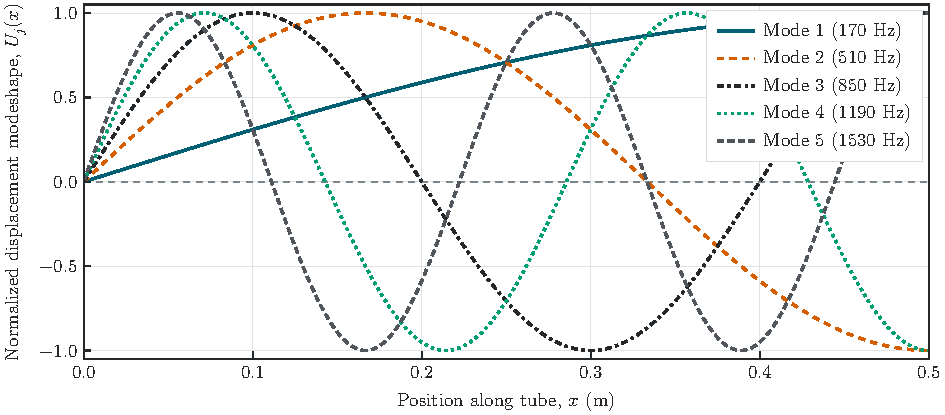
\includegraphics[width=0.96\linewidth]{figures/generated/solutions/C3-closed-open-displacement.pdf}
\caption{Closed--open displacement modeshapes for $L=0.500\,\mathrm{m}$. Legend frequencies identify the five modes.}
\label{fig:hw02-c3-closed-open-disp}
\end{figure}

\textbf{4(i). Comparison with B.4.} B.4 has $z_j=j\pi$ and $f_j=340j\,\mathrm{Hz}$. The closed--open fundamental is half as large, $170\,\mathrm{Hz}$, and only its odd harmonics occur. Both tubes have a displacement node and pressure antinode at $x=0$. Opening the right end replaces the B.4 displacement node with an antinode and its pressure antinode with a node.

The closed--open mode $j$ has $j$ displacement nodes including the closed end and $j$ antinodes including the open end. Its pressure field has $j$ nodes including the open end and $j$ antinodes including the closed end. B.4 instead has $j+1$ displacement nodes including both ends and $j$ interior antinodes; its pressure field has $j$ interior nodes and $j+1$ antinodes including both ends.

\textbf{5(i). Graduate work.} Let $a_j>0$ be the displacement amplitude in meters. Differentiating the displacement field in $p=-K u_x$ gives
\[
p_j(x,t)=-K a_j\gamma_j\cos(\gamma_jx)e^{-i\omega_jt}.
\]
Normalizing by the positive pressure scale $K a_j\gamma_j$ gives
\[
\boxed{\bar{P}_j(x)=-\cos(\gamma_jx)=-\cos\left(\frac{(2j-1)\pi x}{2L}\right)}.
\]
The normalized pressure modeshapes are shown in Figure~\ref{fig:hw02-c3-closed-open-pressure}. The pressure and displacement fields are quarter-cycle shifted because pressure is proportional to the negative spatial derivative of displacement. The closed end is a pressure antinode and displacement node, while the open end is a pressure node and displacement antinode.

\begin{figure}[H]
\centering
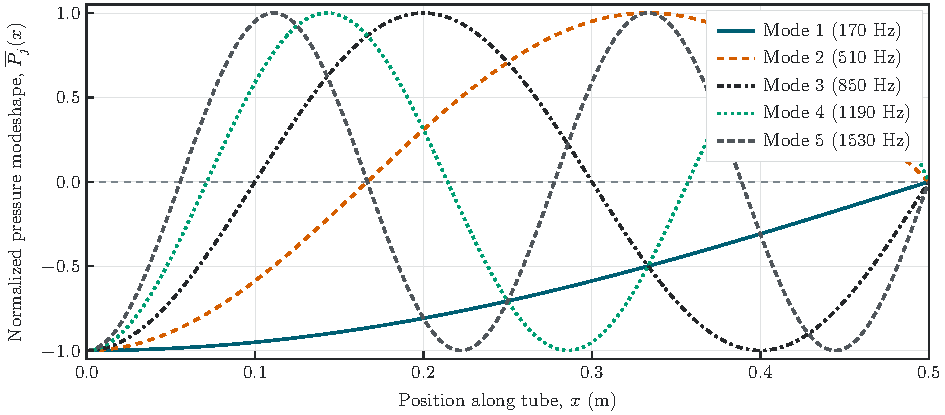
\includegraphics[width=0.96\linewidth]{figures/generated/solutions/C3-closed-open-pressure.pdf}
\caption{Closed--open normalized pressure modeshapes $\bar{P}_j(x)$ for $L=0.500\,\mathrm{m}$.}
\label{fig:hw02-c3-closed-open-pressure}
\end{figure}

\textbf{2(ii). Open--open tube.} The boundary conditions are
\[
p(0,t)=0,\qquad p(L,t)=0.
\]
The first condition gives $C_1=0$, and the second then requires $C_2\sin(\gamma L)=0$. The positive nontrivial roots are
\[
\boxed{z_j=j\pi},\qquad
\boxed{\gamma_j=\frac{j\pi}{L}},\qquad
\boxed{\omega_j=c\gamma_j},\qquad
\boxed{f_j=\frac{jc}{2L}}.
\]
The zero root is a rigid, zero-frequency displacement and is excluded from the acoustic mode index. The first five acoustic modes are
\begin{table}[H]
\centering
\caption{Open--open modal vibration characteristics.}
\label{tab:hw02-c3-open-open}
\small
\begin{tabular}{@{}ccccc@{}}
\toprule
Mode $j$ & $z_j$ (rad) & $\gamma_j$ (rad/m) & $\omega_j$ (krad/s) & $f_j$ (Hz) \\
\midrule
1 & $\pi\approx3.14$ & $6.28$ & $2.14$ & $340$ \\
2 & $2\pi\approx6.28$ & $12.57$ & $4.27$ & $680$ \\
3 & $3\pi\approx9.42$ & $18.85$ & $6.41$ & $1020$ \\
4 & $4\pi\approx12.57$ & $25.1$ & $8.55$ & $1360$ \\
5 & $5\pi\approx15.71$ & $31.4$ & $10.68$ & $1700$ \\
\bottomrule
\end{tabular}
\end{table}

\textbf{3(ii). Displacement modeshapes.} Since $C_1=0$, setting the arbitrary displacement scale to one gives
\[
\boxed{U_j(x)=\cos(\gamma_jx)=\cos\left(\frac{j\pi x}{L}\right)},\qquad j=1,\ldots,5.
\]
The first five physical-length modeshapes are shown in Figure~\ref{fig:hw02-c3-open-open-disp}.

\begin{figure}[H]
\centering
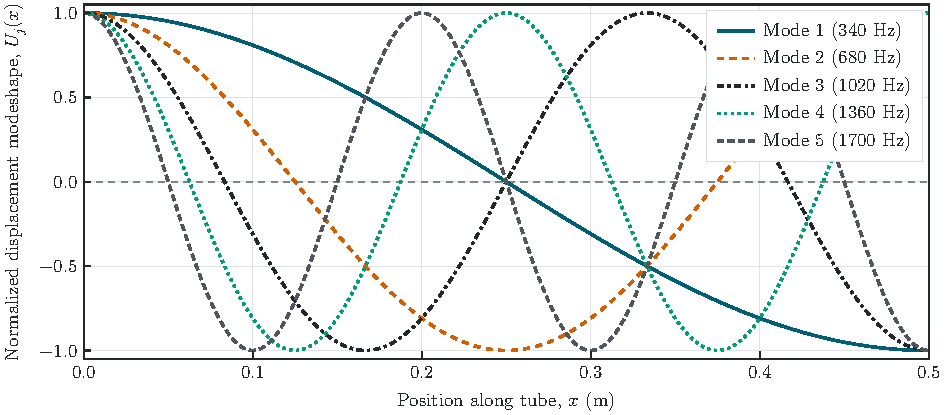
\includegraphics[width=0.96\linewidth]{figures/generated/solutions/C3-open-open-displacement.pdf}
\caption{Open--open displacement modeshapes for $L=0.500\,\mathrm{m}$. Legend frequencies identify the five modes.}
\label{fig:hw02-c3-open-open-disp}
\end{figure}

\textbf{4(ii). Comparison with B.4.} The open--open tube has the same eigenvalues, wavenumbers, and frequencies as B.4. Its cosine displacement and sine pressure shapes are shifted spatially by a quarter-wavelength from the B.4 sine displacement and negative-cosine pressure shapes. Both open ends are displacement antinodes and pressure nodes, reversing the B.4 endpoint roles.

Mode $j$ has $j$ interior displacement nodes and $j+1$ displacement antinodes including both ends. Its pressure field has $j+1$ nodes including both ends and $j$ interior antinodes. B.4 has $j+1$ displacement nodes including both ends and $j$ interior antinodes, with these counts reversed for pressure.

\textbf{5(ii). Graduate work.} Differentiating $U_j(x)$ gives
\[
p_j(x,t)=K a_j\gamma_j\sin(\gamma_jx)e^{-i\omega_jt}.
\]
Normalizing by the positive pressure scale $K a_j\gamma_j$ gives
\[
\boxed{\bar{P}_j(x)=\sin(\gamma_jx)=\sin\left(\frac{j\pi x}{L}\right)}.
\]
The normalized pressure modeshapes are shown in Figure~\ref{fig:hw02-c3-open-open-pressure}. The open ends are pressure nodes and displacement antinodes. The pressure field remains the spatial derivative relation $p=-K u_x$, so the positive sign follows from differentiating the cosine displacement shape.

\begin{figure}[H]
\centering
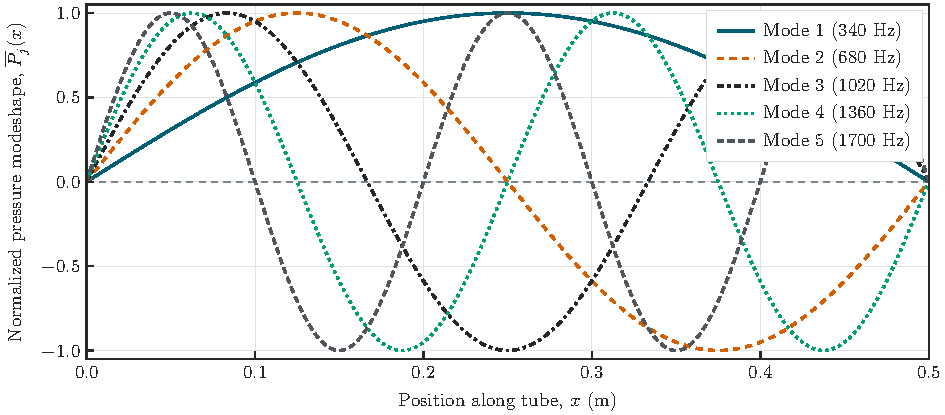
\includegraphics[width=0.96\linewidth]{figures/generated/solutions/C3-open-open-pressure.pdf}
\caption{Open--open normalized pressure modeshapes $\bar{P}_j(x)$ for $L=0.500\,\mathrm{m}$.}
\label{fig:hw02-c3-open-open-pressure}
\end{figure}

\clearpage
\matlabcaption{MATLAB calculations and plots for C.3.}
\lstinputlisting[style=hwmatlab]{matlab/C3.m}

\end{document}
